% Options for packages loaded elsewhere
% Options for packages loaded elsewhere
\PassOptionsToPackage{unicode}{hyperref}
\PassOptionsToPackage{hyphens}{url}
\PassOptionsToPackage{dvipsnames,svgnames,x11names}{xcolor}
%
\documentclass[
  letterpaper,
  DIV=11,
  numbers=noendperiod,
  oneside]{scrartcl}
\usepackage{xcolor}
\usepackage[left=1in,marginparwidth=2.0666666666667in,textwidth=4.1333333333333in,marginparsep=0.3in]{geometry}
\usepackage{amsmath,amssymb}
\setcounter{secnumdepth}{-\maxdimen} % remove section numbering
\usepackage{iftex}
\ifPDFTeX
  \usepackage[T1]{fontenc}
  \usepackage[utf8]{inputenc}
  \usepackage{textcomp} % provide euro and other symbols
\else % if luatex or xetex
  \usepackage{unicode-math} % this also loads fontspec
  \defaultfontfeatures{Scale=MatchLowercase}
  \defaultfontfeatures[\rmfamily]{Ligatures=TeX,Scale=1}
\fi
\usepackage{lmodern}
\ifPDFTeX\else
  % xetex/luatex font selection
\fi
% Use upquote if available, for straight quotes in verbatim environments
\IfFileExists{upquote.sty}{\usepackage{upquote}}{}
\IfFileExists{microtype.sty}{% use microtype if available
  \usepackage[]{microtype}
  \UseMicrotypeSet[protrusion]{basicmath} % disable protrusion for tt fonts
}{}
\makeatletter
\@ifundefined{KOMAClassName}{% if non-KOMA class
  \IfFileExists{parskip.sty}{%
    \usepackage{parskip}
  }{% else
    \setlength{\parindent}{0pt}
    \setlength{\parskip}{6pt plus 2pt minus 1pt}}
}{% if KOMA class
  \KOMAoptions{parskip=half}}
\makeatother
% Make \paragraph and \subparagraph free-standing
\makeatletter
\ifx\paragraph\undefined\else
  \let\oldparagraph\paragraph
  \renewcommand{\paragraph}{
    \@ifstar
      \xxxParagraphStar
      \xxxParagraphNoStar
  }
  \newcommand{\xxxParagraphStar}[1]{\oldparagraph*{#1}\mbox{}}
  \newcommand{\xxxParagraphNoStar}[1]{\oldparagraph{#1}\mbox{}}
\fi
\ifx\subparagraph\undefined\else
  \let\oldsubparagraph\subparagraph
  \renewcommand{\subparagraph}{
    \@ifstar
      \xxxSubParagraphStar
      \xxxSubParagraphNoStar
  }
  \newcommand{\xxxSubParagraphStar}[1]{\oldsubparagraph*{#1}\mbox{}}
  \newcommand{\xxxSubParagraphNoStar}[1]{\oldsubparagraph{#1}\mbox{}}
\fi
\makeatother


\usepackage{longtable,booktabs,array}
\usepackage{calc} % for calculating minipage widths
% Correct order of tables after \paragraph or \subparagraph
\usepackage{etoolbox}
\makeatletter
\patchcmd\longtable{\par}{\if@noskipsec\mbox{}\fi\par}{}{}
\makeatother
% Allow footnotes in longtable head/foot
\IfFileExists{footnotehyper.sty}{\usepackage{footnotehyper}}{\usepackage{footnote}}
\makesavenoteenv{longtable}
\usepackage{graphicx}
\makeatletter
\newsavebox\pandoc@box
\newcommand*\pandocbounded[1]{% scales image to fit in text height/width
  \sbox\pandoc@box{#1}%
  \Gscale@div\@tempa{\textheight}{\dimexpr\ht\pandoc@box+\dp\pandoc@box\relax}%
  \Gscale@div\@tempb{\linewidth}{\wd\pandoc@box}%
  \ifdim\@tempb\p@<\@tempa\p@\let\@tempa\@tempb\fi% select the smaller of both
  \ifdim\@tempa\p@<\p@\scalebox{\@tempa}{\usebox\pandoc@box}%
  \else\usebox{\pandoc@box}%
  \fi%
}
% Set default figure placement to htbp
\def\fps@figure{htbp}
\makeatother





\setlength{\emergencystretch}{3em} % prevent overfull lines

\providecommand{\tightlist}{%
  \setlength{\itemsep}{0pt}\setlength{\parskip}{0pt}}



 


% load packages
\usepackage{geometry}
\usepackage{xcolor}
\usepackage{eso-pic}
\usepackage{fancyhdr}
\usepackage{sectsty}
\usepackage{fontspec}
\usepackage{titlesec}

%% Set page size with a wider right margin
\geometry{a4paper, total={170mm,257mm}, left=20mm, top=20mm, bottom=20mm, right=50mm}

%% Let's define some colours
\definecolor{light}{HTML}{E6E6FA}
\definecolor{highlight}{HTML}{800080}
\definecolor{dark}{HTML}{330033}

% %% Let's add the border on the right hand side 
% \AddToShipoutPicture{% 
%     \AtPageLowerLeft{% 
%         \put(\LenToUnit{\dimexpr\paperwidth-3cm},0){% 
%             \color{light}\rule{3cm}{\LenToUnit\paperheight}%
%           }%
%      }%
%      % logo
%     \AtPageLowerLeft{% start the bar at the bottom right of the page
%         \put(\LenToUnit{\dimexpr\paperwidth-2.25cm},27.2cm){% move it to the top right
%             \color{light}
\includegraphics[width=1.5cm]{_extensions/nrennie/PrettyPDF/logo.png}
%           }%
%      }%
% }

%% Style the page number
\fancypagestyle{mystyle}{
  \fancyhf{}
  \renewcommand\headrulewidth{0pt}
  \fancyfoot[R]{\thepage}
  \fancyfootoffset{3.5cm}
}
\setlength{\footskip}{20pt}

%% style the chapter/section fonts
\chapterfont{\color{dark}\fontsize{20}{16.8}\selectfont}
\sectionfont{\color{dark}\fontsize{20}{16.8}\selectfont}
\subsectionfont{\color{dark}\fontsize{14}{16.8}\selectfont}
\titleformat{\subsection}
  {\sffamily\Large\bfseries}{\thesection}{1em}{}[{\titlerule[0.8pt]}]
  
% left align title
\makeatletter
\renewcommand{\maketitle}{\bgroup\setlength{\parindent}{0pt}
\begin{flushleft}
  {\sffamily\huge\textbf{\MakeUppercase{\@title}}} \vspace{0.3cm} \newline
  {\Large {\@subtitle}} \newline
  \@author
\end{flushleft}\egroup
}
\makeatother

%% Use some custom fonts
\setsansfont{Ubuntu}[
    Path=_extensions/nrennie/PrettyPDF/Ubuntu/,
    Scale=0.9,
    Extension = .ttf,
    UprightFont=*-Regular,
    BoldFont=*-Bold,
    ItalicFont=*-Italic,
    ]

\setmainfont{Ubuntu}[
    Path=_extensions/nrennie/PrettyPDF/Ubuntu/,
    Scale=0.9,
    Extension = .ttf,
    UprightFont=*-Regular,
    BoldFont=*-Bold,
    ItalicFont=*-Italic,
    ]
\KOMAoption{captions}{tableheading}
\makeatletter
\@ifpackageloaded{caption}{}{\usepackage{caption}}
\AtBeginDocument{%
\ifdefined\contentsname
  \renewcommand*\contentsname{Table of contents}
\else
  \newcommand\contentsname{Table of contents}
\fi
\ifdefined\listfigurename
  \renewcommand*\listfigurename{List of Figures}
\else
  \newcommand\listfigurename{List of Figures}
\fi
\ifdefined\listtablename
  \renewcommand*\listtablename{List of Tables}
\else
  \newcommand\listtablename{List of Tables}
\fi
\ifdefined\figurename
  \renewcommand*\figurename{Figure}
\else
  \newcommand\figurename{Figure}
\fi
\ifdefined\tablename
  \renewcommand*\tablename{Table}
\else
  \newcommand\tablename{Table}
\fi
}
\@ifpackageloaded{float}{}{\usepackage{float}}
\floatstyle{ruled}
\@ifundefined{c@chapter}{\newfloat{codelisting}{h}{lop}}{\newfloat{codelisting}{h}{lop}[chapter]}
\floatname{codelisting}{Listing}
\newcommand*\listoflistings{\listof{codelisting}{List of Listings}}
\makeatother
\makeatletter
\makeatother
\makeatletter
\@ifpackageloaded{caption}{}{\usepackage{caption}}
\@ifpackageloaded{subcaption}{}{\usepackage{subcaption}}
\makeatother
\makeatletter
\@ifpackageloaded{tcolorbox}{}{\usepackage[skins,breakable]{tcolorbox}}
\makeatother
\makeatletter
\@ifundefined{shadecolor}{\definecolor{shadecolor}{rgb}{.97, .97, .97}}{}
\makeatother
\makeatletter
\@ifundefined{codebgcolor}{\definecolor{codebgcolor}{named}{light}}{}
\makeatother
\makeatletter
\ifdefined\Shaded\renewenvironment{Shaded}{\begin{tcolorbox}[sharp corners, breakable, enhanced, frame hidden, colback={codebgcolor}, boxrule=0pt]}{\end{tcolorbox}}\fi
\makeatother
\makeatletter
\@ifpackageloaded{sidenotes}{}{\usepackage{sidenotes}}
\@ifpackageloaded{marginnote}{}{\usepackage{marginnote}}
\makeatother
\usepackage{bookmark}
\IfFileExists{xurl.sty}{\usepackage{xurl}}{} % add URL line breaks if available
\urlstyle{same}
\hypersetup{
  pdftitle={Bookish},
  colorlinks=true,
  linkcolor={highlight},
  filecolor={Maroon},
  citecolor={Blue},
  urlcolor={highlight},
  pdfcreator={LaTeX via pandoc}}


\title{Bookish}
\usepackage{etoolbox}
\makeatletter
\providecommand{\subtitle}[1]{% add subtitle to \maketitle
  \apptocmd{\@title}{\par {\large #1 \par}}{}{}
}
\makeatother
\subtitle{Bibliomania and the Social Life of Reading}
\author{}
\date{}
\begin{document}
\maketitle

\pagestyle{mystyle}


\href{https://shesbecomingbookish.com/}{\pandocbounded{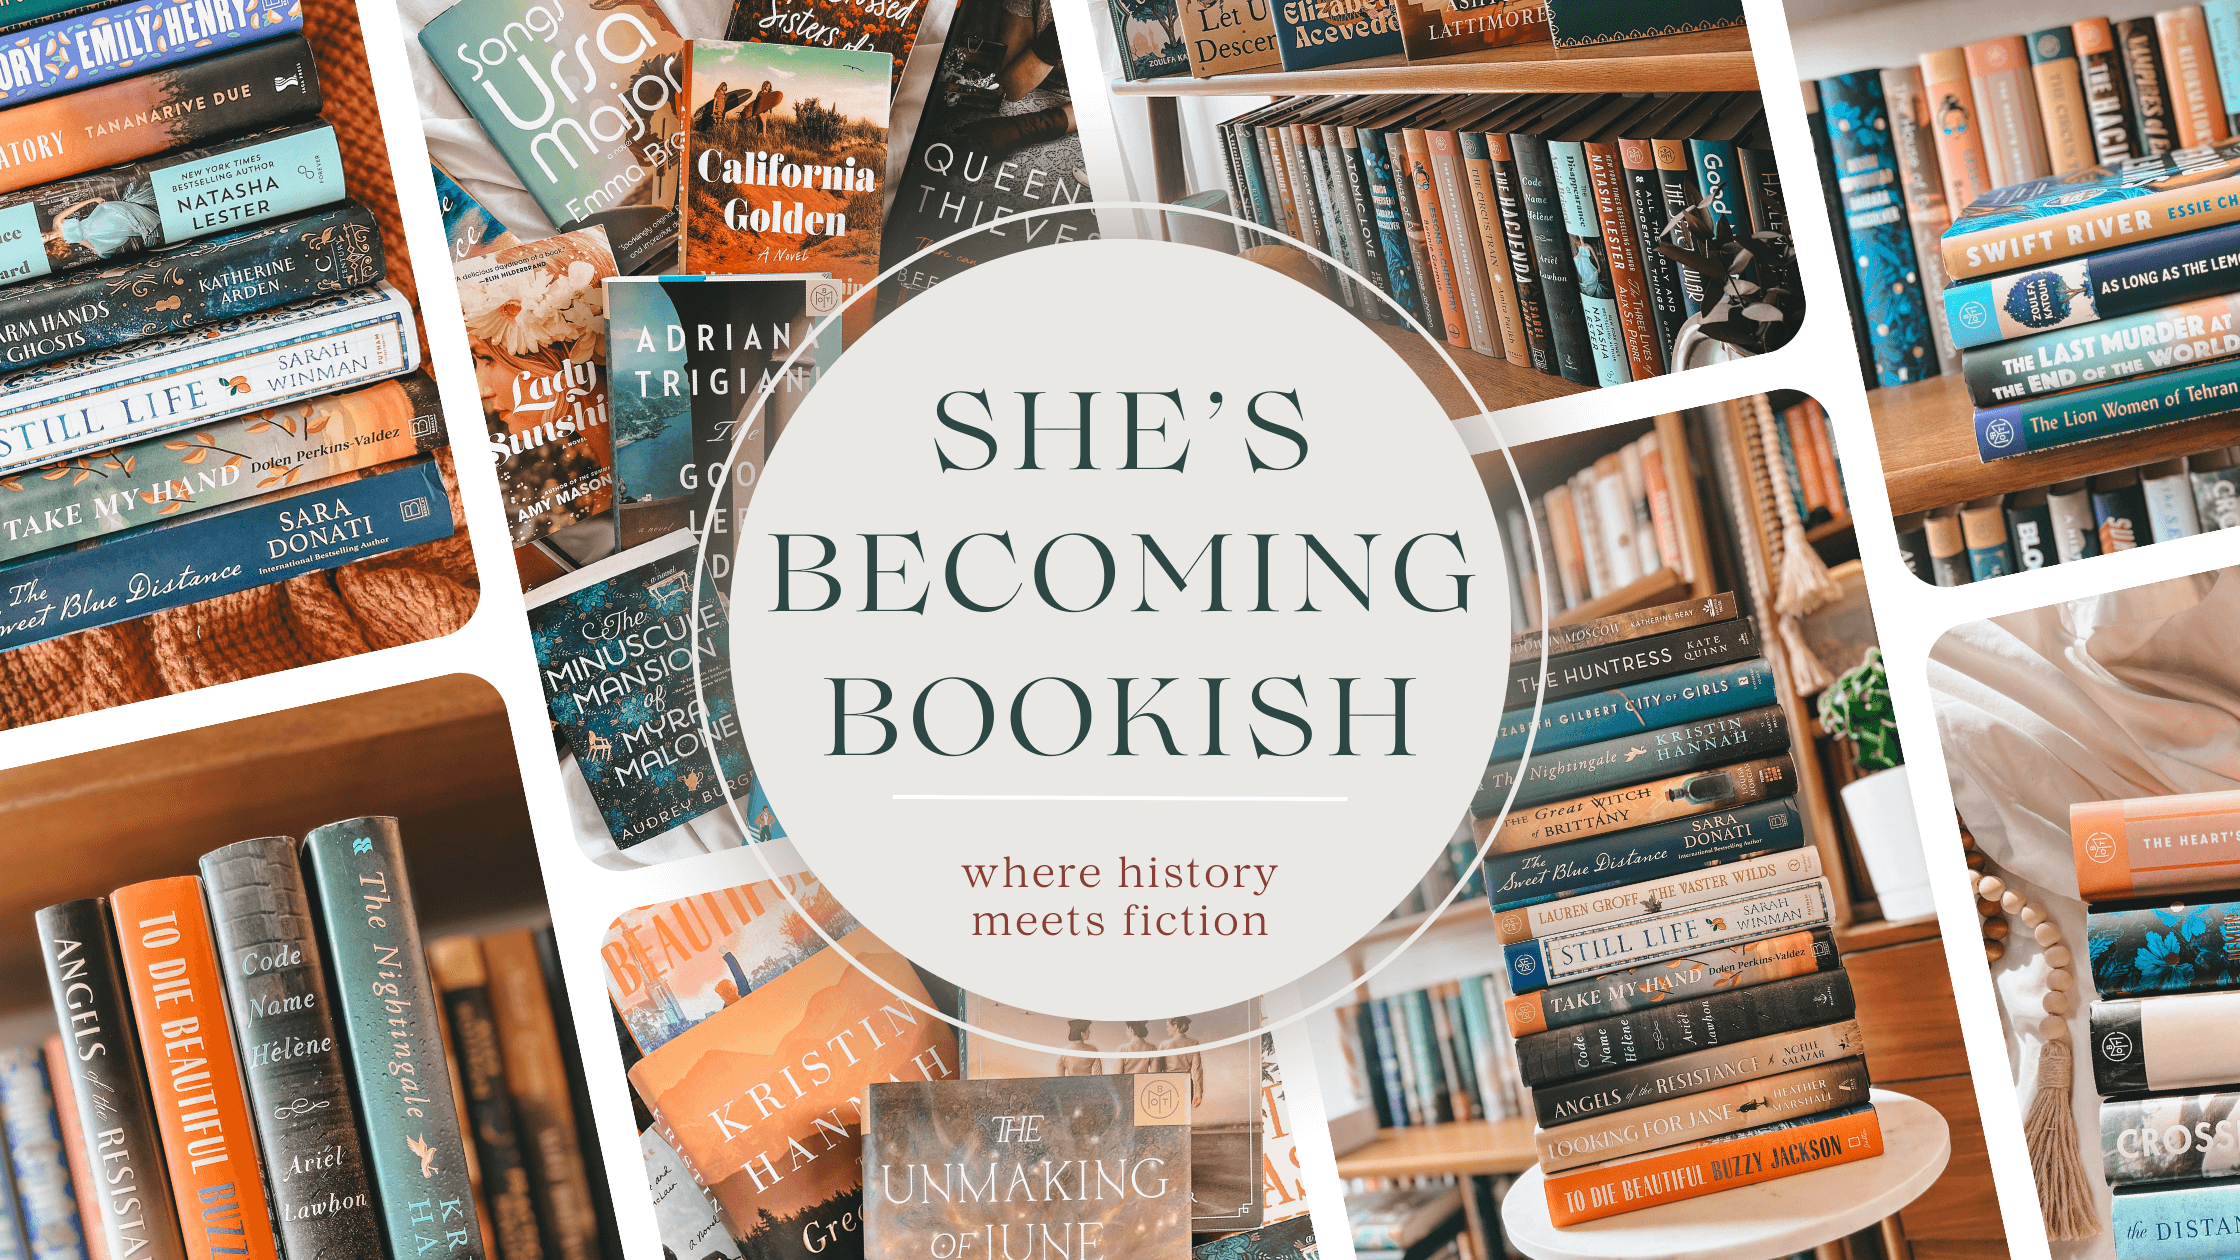
\includegraphics[keepaspectratio]{img/bookish.png}}}

\marginnote{\begin{footnotesize}

Jessica Maddox and Fiona Gill,
``\href{https://journals.sagepub.com/doi/epub/10.1177/20563051231213565}{Assembling
`Sides' of TikTok: Examining Community, Culture, and Interface through a
BookTok Case Study}''José M. Tomasena,
``\href{https://journals.sagepub.com/doi/epub/10.1177/2056305119894004}{Negotiating
Collaborations: BookTubers, The Publishing Industry, and YouTube's
Ecosystem}''

See also:

Alysia De Melo,
``\href{https://journals.sagepub.com/doi/epub/10.1177/20563051241286700}{The
Influence of BookTok on Literary Criticisms and Diversity}''Michael
Dezuanni and Amy Schoonens,
``\href{https://journals.sagepub.com/doi/epub/10.1177/20563051241309499}{\#BookTok's
Peer Pedagogies: Invitations to Learn About Books and Reading on
TikTok}''D. Bondy Valdovinos Kaye,
``\href{https://watermark.silverchair.com/92kaye.pdf?token=AQECAHi208BE49Ooan9kkhW_Ercy7Dm3ZL_9Cf3qfKAc485ysgAAA0IwggM-BgkqhkiG9w0BBwagggMvMIIDKwIBADCCAyQGCSqGSIb3DQEHATAeBglghkgBZQMEAS4wEQQMUQ3G4vO_yq2mYcrPAgEQgIIC9cFNcqJ-tvkfDkABZcgdqxRKk2nBHZwwo0JsNBv506DO0UmmiXXZMCVhjbGJulFTAD9GNWkNkMkdGiceXop6meQPzGcowi2352fEas53GVIEP6OfBSz7nGE3GDB5HeOgxIaNlYoBpu4eOkZuT9ylyL9nyJnLW728HsU6PoXyAzmvO21RZthx1-VDaii8db72kmS9SX754tbugG5z97yra1Vr7ZDZHcM6lWv_ot5YjNfgHX_YI0LUTbgorUsAS374e6ovCundjdohOPc0EzGKKsH3oB1TJ8t7KKM6-OUlGIhkNfHUZW27SwEHe9cysKfwKnIh2J3MdKs_Vb_5uq_glDkntrxoIaLL_H_ygoOhPpIUfeXhkaeCVTydh-Z81oOjo5T_d7wHLqmPGFR4ury1BQSv47KFmWcWNnamBqUOFqbe1sXZsjF4-LAjoTqERwmjA8KowI9oR8X6O0uFgfPL7X0lWa_WhIsTWiKtmHyOpteJeOmlSU63bf4KAPox_9SU0YahHIK1pd9hEfp7vY4h7zE88EYj9L8e_aTa37rNtt165htvmcuVE8Ed_9qCZghryDIy93hjLbBUIQbQvC_t-kv2PCYQRAkx7HjSIGnTqSogR0H8oxUX00LgHdfjqQF6LZoju0qhFfKyEbzWniLxr-iHZ4ESt6jgve5KGYDQNLVe9FZmeGMEayInt4izRmhvdunONM2nkhdeIYlDAaIoyfqIDXUqupLP1V_V6vGMVVb1-IY6RjGsj-T8TL4fM4K8WQT9LtytSmm2LXbqTH7QF91OoYcN-8_0WtY1UGr7KbRdg5bqKQpYQw5os3TpXOiNgS81QkP25iy-bQS4HU_d6jtubjXgcYYeHR_tNVTyY3ldUMiEKoJwAOKShlIzlAsc1LC0-e3VurvTPnyRkvZiSclNDceco2aUwR6Ld6WxexZvyltprjN5wxYBIx2k9EfnmXXiOYyMOswMU4ICOZEaw4Ba6qg7rfCTO4P6P1P3hSjS5jBakZY}{JazzTok:
Creativity, Community, and Improvisation on TikTok},'' \textbf{Jazz and
Culture} 6 (2) (2023): 92--116.

\end{footnotesize}}

\begin{quote}
\emph{Bookstagram is known for its luxurious aesthetic celebrating the
materiality of books \ldots{} This bookish aesthetic is developed in
posts that feature beautifully styled books and bookish objects as well
as posts that celebrate reading as desirable activity.}

---Bronwyn Reddan,
``\href{http://www.slav.vic.edu.au/index.php/Synergy/article/view/597}{Social
reading cultures on BookTube, Bookstagram, and BookTok}
\end{quote}

Are you ``bookish''? As you'll have seen if you've read Jessica Maddox
and Fiona Gill's article this week about Booktok (and maybe looked more
closely at its references), the term has become ubiquitous in the
intersecting worlds of Booktube, Bookstagram, and Booktok, as well as
social reading sites like \href{https://www.goodreads.com/}{Goodreads}.
I want to spend some time here reflecting on the concept of
\textbf{bookishness} itself. What does it mean to be, or to become,
``bookish'' anyway? While the term itself long predates social media, of
course, it's taken on a particular meaning and a particular
\textbf{resonance} in relation to the representation of books and the
practice of reading on social media. In that context, to be ``bookish''
means quite specifically to participate in what Maddox and Gill refer to
as the ``digital imagined community'' of bibliophiles extending across
the social media platforms of YouTube, Instagram, and TikTok. So what
does being ``bookish'' actually mean in that specific context? What
exactly is ``bookishness'' in the context of social media?

We could start with the term's rather odd suffix: \emph{ish}. In popular
usage, the term ``-ish'' suggests an \textbf{approximation} to something
rather than precise definition. ``Let's meet at six-ish'' means that
we'll meet \textbf{around} 18:00 hours but not necessarily exactly at
that time. But as you know, it's quite common now in everyday
conversation to use the ending ``-ish'' on its own, detached from a
preceding noun, as a kind of shorthand to refer to an approximate state
or emotion: ``So did you enjoy the movie?'' ---``Ish''.

To be book\textbf{ish}, then, suggests a looser, more casual affiliation
with books and compared to that of the professional critic, academic
literature scholor, publisher, bookseller, or author. It invokees
amateur appreciation rather than scholarly expertise, pleasure rather
than literary analysis. Yet because of the high cultural prestige
attached to books (what the social theorist Pierre Bourdieu calls
symbolic capital) that remains attached to books, to identify as
``bookish'' is still to claim or perform a certain form of social
\textbf{distinction}. In the social media realm, then, ``bookishness''
becomes a form of non-specialized (at least in the academic sense of
specialization) social identity defined---I would argue---not by
disciplinary expertise (textual analysis, historical knowledge) but
defined purely and simply by an \textbf{affective} relation to its
object: what's often referred to as a \textbf{passion} for books and
reading. From this standpoint, we can say first of all that
``bookishness'' is a form of \textbf{fandom}, and we know how the
popular knowledge of fans involves a very different (I would say
affective) relation to its object rather than the \textbf{dispassionate}
position required of the literary scholar.

What's equally clear from both of the primary reading assignments for
this week is that ``bookishness'' as a social (media) identity involves
not just an affective relation to its object but also a commodified one,
that of a \textbf{consumer}. It's no coincidence that the most common
video format of Booktubers and Booktok creators is the
\textbf{recommendation video}, with recommendation here involving not
just the question of whether a book is worth your time but also your
money. As José Miguel Tomasena explains in his article, Booktubers on
YouTube and other social platforms play a crucial role in the
circulation and promotion of books and authors, similar to that of music
or film critics, in a similar way to how fashion or beauty bloggers
become ``brand ambassadors''. In addition to their overtly commercial
role, though, Booktubers also embody the fantasy of ``bookishness''
through their conspicuous consumption (a term coined by Thorstein Veblen
more than a century ago) through their fetishizing of books as material
objects and their highly stylized performances and indeed staging of
bibliophilia (literally the love of books). In her brilliant analysis of
this phenomenon, Bronwyn Radden refers to this as ``a bookish
\textbf{aesthetic},'' and this aestheticization of books and the
practice of reading itself into a self-consciously performed ritual
invokes the sociological concept of \textbf{lifestyle}, which could be
defined as a form of modern social identity in which in capitalism the
modern self is articulated exclusively through commodities and
consumption.

This bring me to my last point, about \textbf{aesthetics}---a concept
that we will be focusing on in depth in the last week of the course. For
now, let me conclude by defining ``bookishness'' as what in social media
parlance today is known as an \textbf{aesthetic}. If we consider
bookishness in this way, we can see that there are two quite distinct
ways of thinking about Booktok. The first is the approach taken by
Jessica Maddox and Fiona Gill in their article, where it is
contextualized as one of the many ``sides'' of TikTok (I've included a
different example of such a ``side'' below, in Queline Meadows's superb
video essay about Film TikTok; there is also a link in the margin to an
article about Jazz TikTok).

The other way of thinking about Booktok, which to me makes more sense
than its ``internal'' relationship to other ``sides'' of TikTok, is to
re-frame it as an aesthetic that is not confined to TikTok but extending
across not only other platforms (notably YouTube, Instagram, Twitter)
but also independent personal blogs such as the one linked to at the
beginning of this page. While the bookish aesthetic takes different
forms on each of these different platforms according to their particular
affordances (YouTube vs.~Insta vs.~TikTok), they do have much in common.
I think it makes more sense to consider bookishness as an **internet
aesthetic* and to consider it comparatively across multiple social media
platforms for that reason. This is even though there are numerous
articles specifically about Booktok in particular, I thought it was
important also to consider the bookish aesthetic not just on TikTok but
also on YouTube (the Tomasena article) and Instagram (the Redden
article, linked at the beginning of this lecture).

My argument here may seem a bit strange at this point, given that we are
so used to thinking about social media vertically, in terms of
\textbf{platform infrastructures}. Even though different platforms may
have the same corporate owner, we still tend to approarch social media
in this way (see the TikTok Research Network). Methodologically, it
makes sense, I suppose, but the drawback is that it may lead us to miss
the bigger picture; the concept of aesthetics enables us to connect the
pieces of the larger jigsaw puzzle.

Hopefully the preceding discussion will make more sense when return to
the topic of aesthetics in the concluding week of the course. For now, I
hope what I've said makes sense and look forward to hearing about your
own relationship to Booktok or the bookish aesthetic on other platforms.

There is, of course, a lot more to say about the larger phenomenon of
the cult of physical books and reading as a backlash against the
domination of digital, virtual, and visual culture. I think it would be
simplistic to reduce it simply to nostalgia for analog culture, though,
since we must remember that the the bookish aesthetic or subculture is
itself a \textbf{networked public} (boyd) or \textbf{digital imagined
community} (Anderson).

I'm embedding and linking some videos and other sources below that
connect both to this readings and my own discussion of them here, and
encourage you to explore them and share your thoughts about them in your
weekly Review post and the discussion channel on Discord.

\begin{center}\rule{0.5\linewidth}{0.5pt}\end{center}

\textbf{Key Concepts}

\begin{itemize}
\tightlist
\item
  ``Side'' (of TikTok)
\item
  Platform vernaculars
\item
  Imitation publics
\item
  Imagined communities
\item
  Recommendation video
\item
  ``Bookish'' aesthetics
\item
  Social/symbolic capital (Bourdieu)
\end{itemize}

\textbf{Further Reading}\\
Claire Armistead,
``\href{https://www.theguardian.com/books/2022/jun/08/lockdown-exploded-tiktok-books-revolution-booktok}{`After
lockdown, things exploded' - how TikTok triggered a books revolution}
(\textbf{The Guardian}, 8 June 2022).\\
Dorothee Birke,''\href{https://doi.org/10.1215/03335372-8883178}{Social
Reading? On the Rise of a `Bookish' Reading Culture Online},''
\textbf{Poetics Today} 42 (2) (2021): 149--172.\\
Bronwyn Reddan,
``\href{http://www.slav.vic.edu.au/index.php/Synergy/article/view/597}{Social
reading cultures on BookTube, Bookstagram, and BookTok},''
\textbf{Synergy}, 20 (1) (2022).\\
\href{https://x.com/bcredibility?lang=en}{Bookcase Credibility}\\

\begin{center}\rule{0.5\linewidth}{0.5pt}\end{center}

\textbf{The Rise of Film TikTok} (kikikrazed/Queline Meadows)

\url{https://youtu.be/iqajurNSp1Q}

\begin{center}\rule{0.5\linewidth}{0.5pt}\end{center}

\textbf{Researching Booktube as a Booktuber}
(\href{https://www.youtube.com/@jmtomasena_}{José Miguel Tomasena})

\url{https://youtu.be/kzysSOvDvGo}

\begin{center}\rule{0.5\linewidth}{0.5pt}\end{center}

\href{https://youtu.be/DwOpkhxexcA}{\textbf{My Honest Thoughts on
Booktok, Over Consumption of Books, Loss of Personal Reading Tastes \&
more}} (\href{https://www.youtube.com/@AnaWallaceJohnson/videos}{Ana
Wallace Johnson})

(Follow link - video not available for embedding)

\begin{center}\rule{0.5\linewidth}{0.5pt}\end{center}

\textbf{Reading for 24 hours straight in a book hotel\ldots{}}
\href{https://www.youtube.com/@haleypham/videos}{Haley Pham}

\url{https://youtu.be/bqaopTTpaP8}

\begin{center}\rule{0.5\linewidth}{0.5pt}\end{center}




\end{document}
